\appendix

\chapter{Model predictions}

\begin{figure}[!htb]
    \centering
    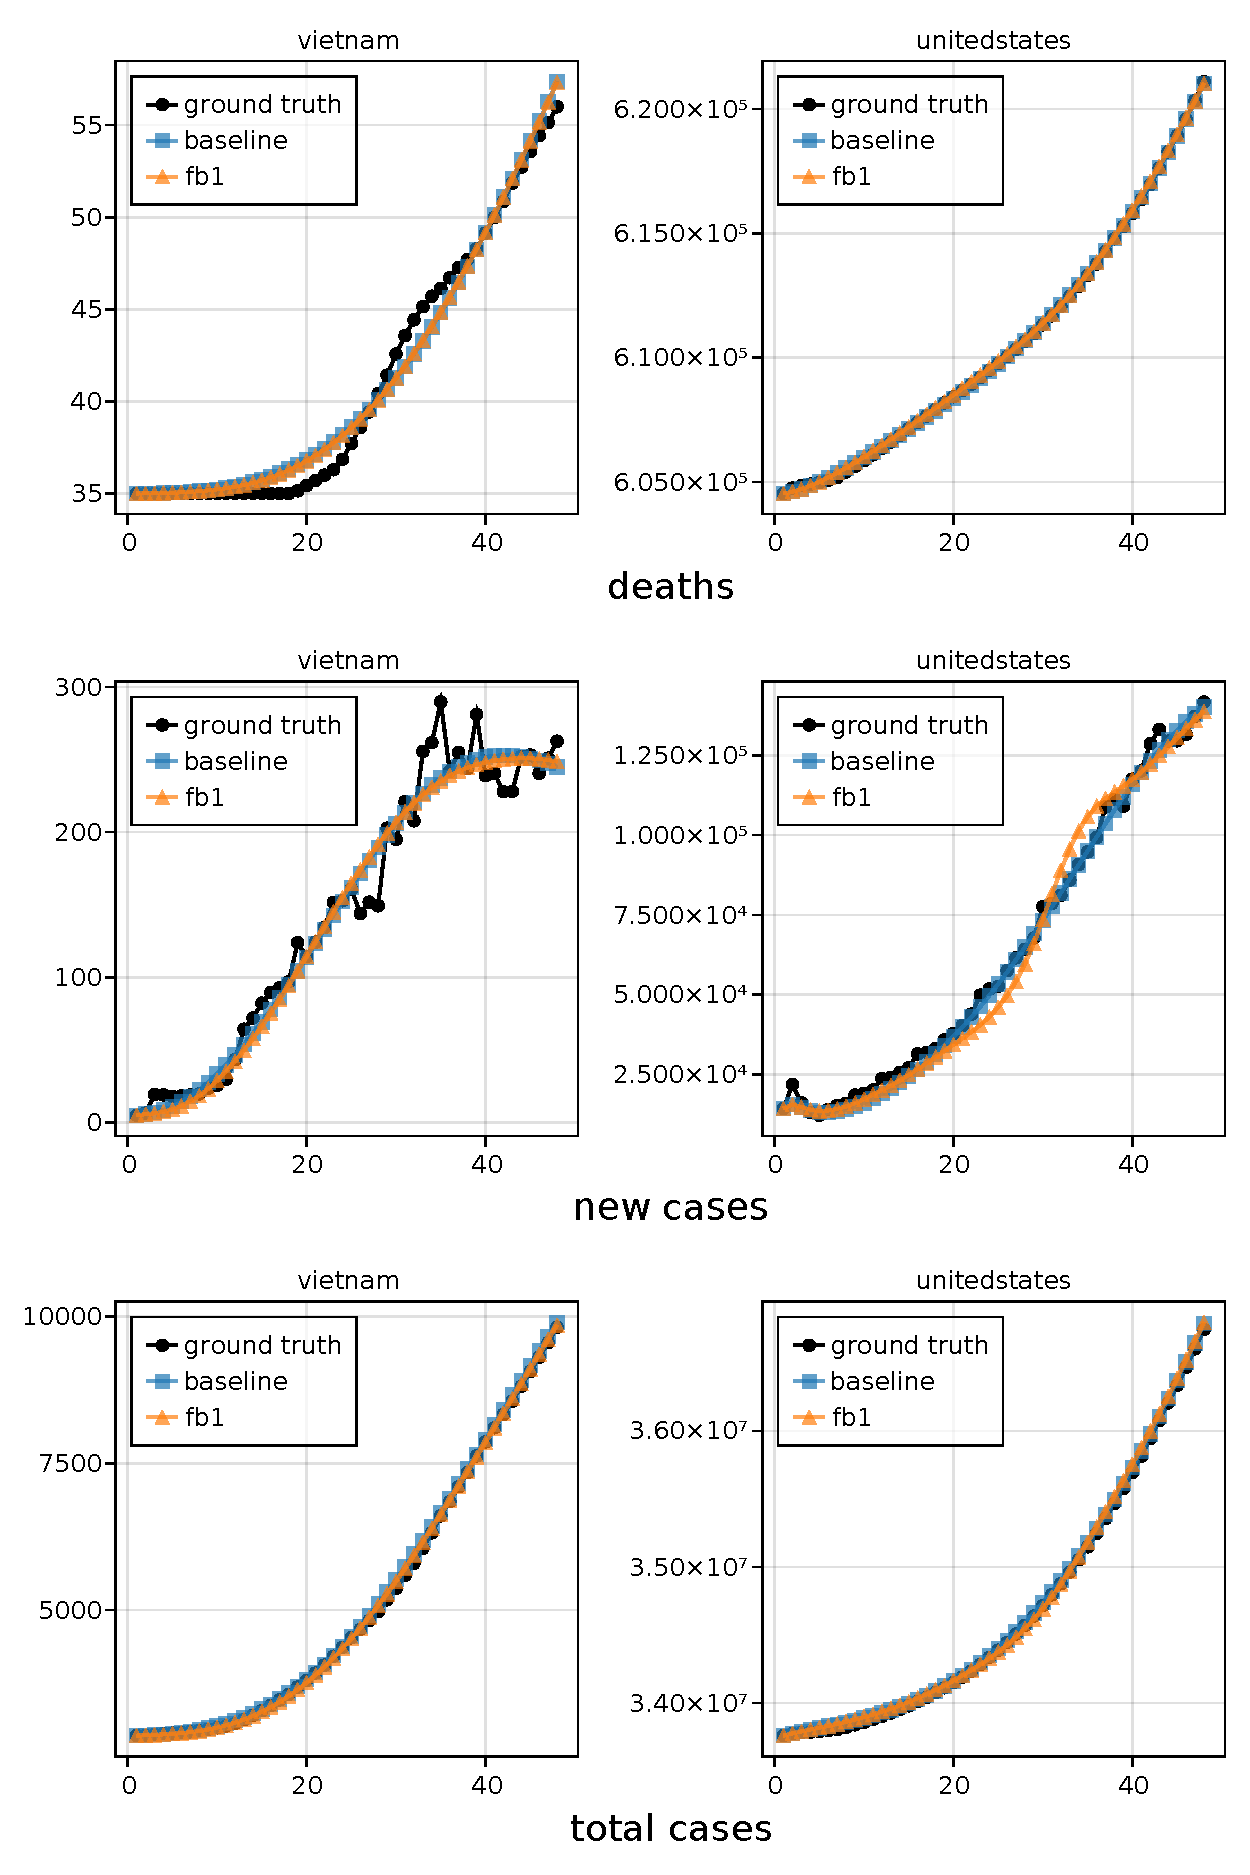
\includegraphics[scale=0.35]{fit_country_level.pdf}
    \caption{Predictions made by all versions of the model for the training period after having trained with country-level data. Each row contains the predictions for a compartment for each of the considered countries. Here the second version is denoted as \textit{fb1}}
    \label{fig:fit-country-level}
\end{figure}

\begin{figure}[!htb]
    \centering
    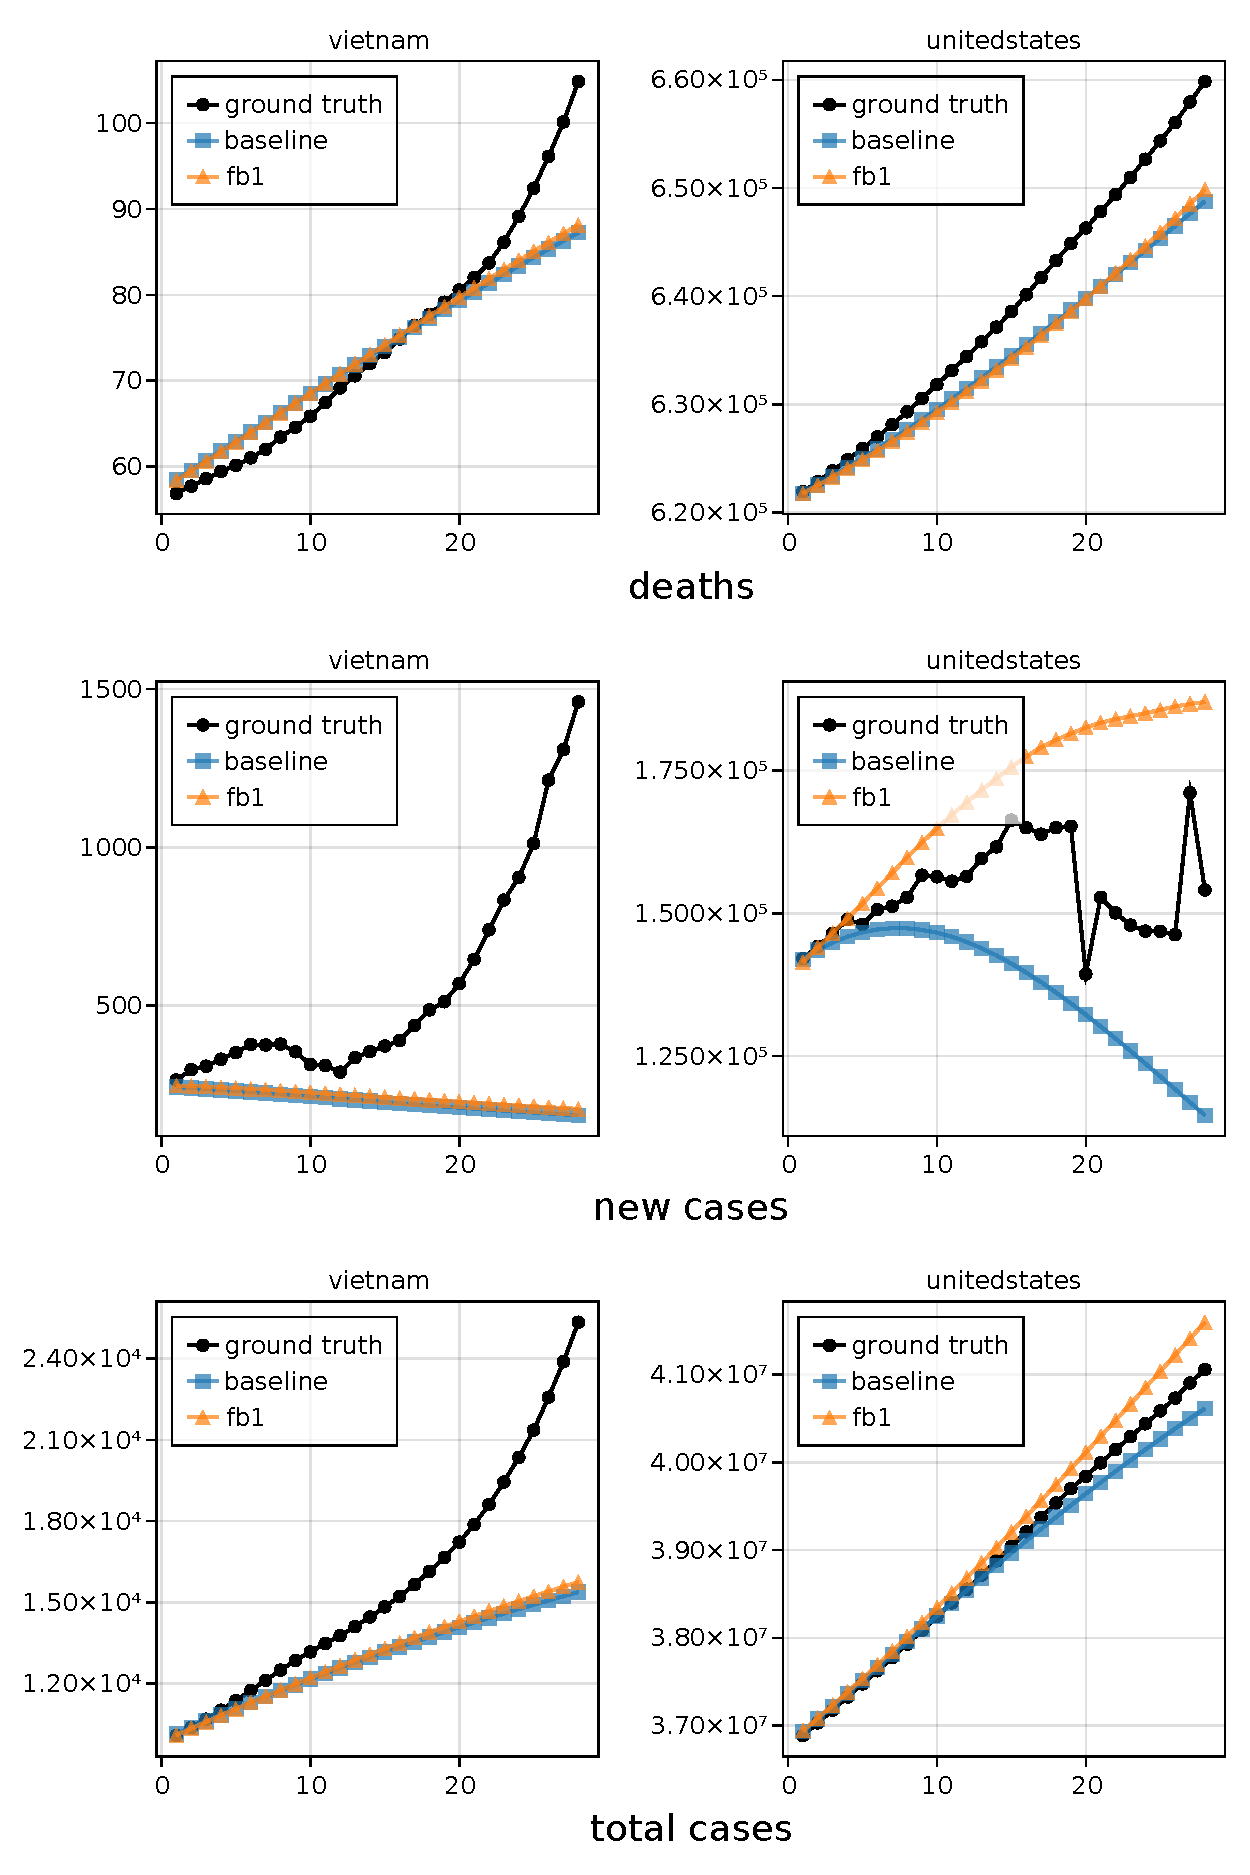
\includegraphics[scale=0.35]{pred_country_level.pdf}
    \caption{Predictions made by all versions of the model for the testing period after having trained with country-level data. Each row contains the predictions for a compartment for each of the considered countries. Here the second version is denoted as \textit{fb1}}
    \label{fig:pred-country-level}
\end{figure}

\begin{figure}[!htb]
    \centering
    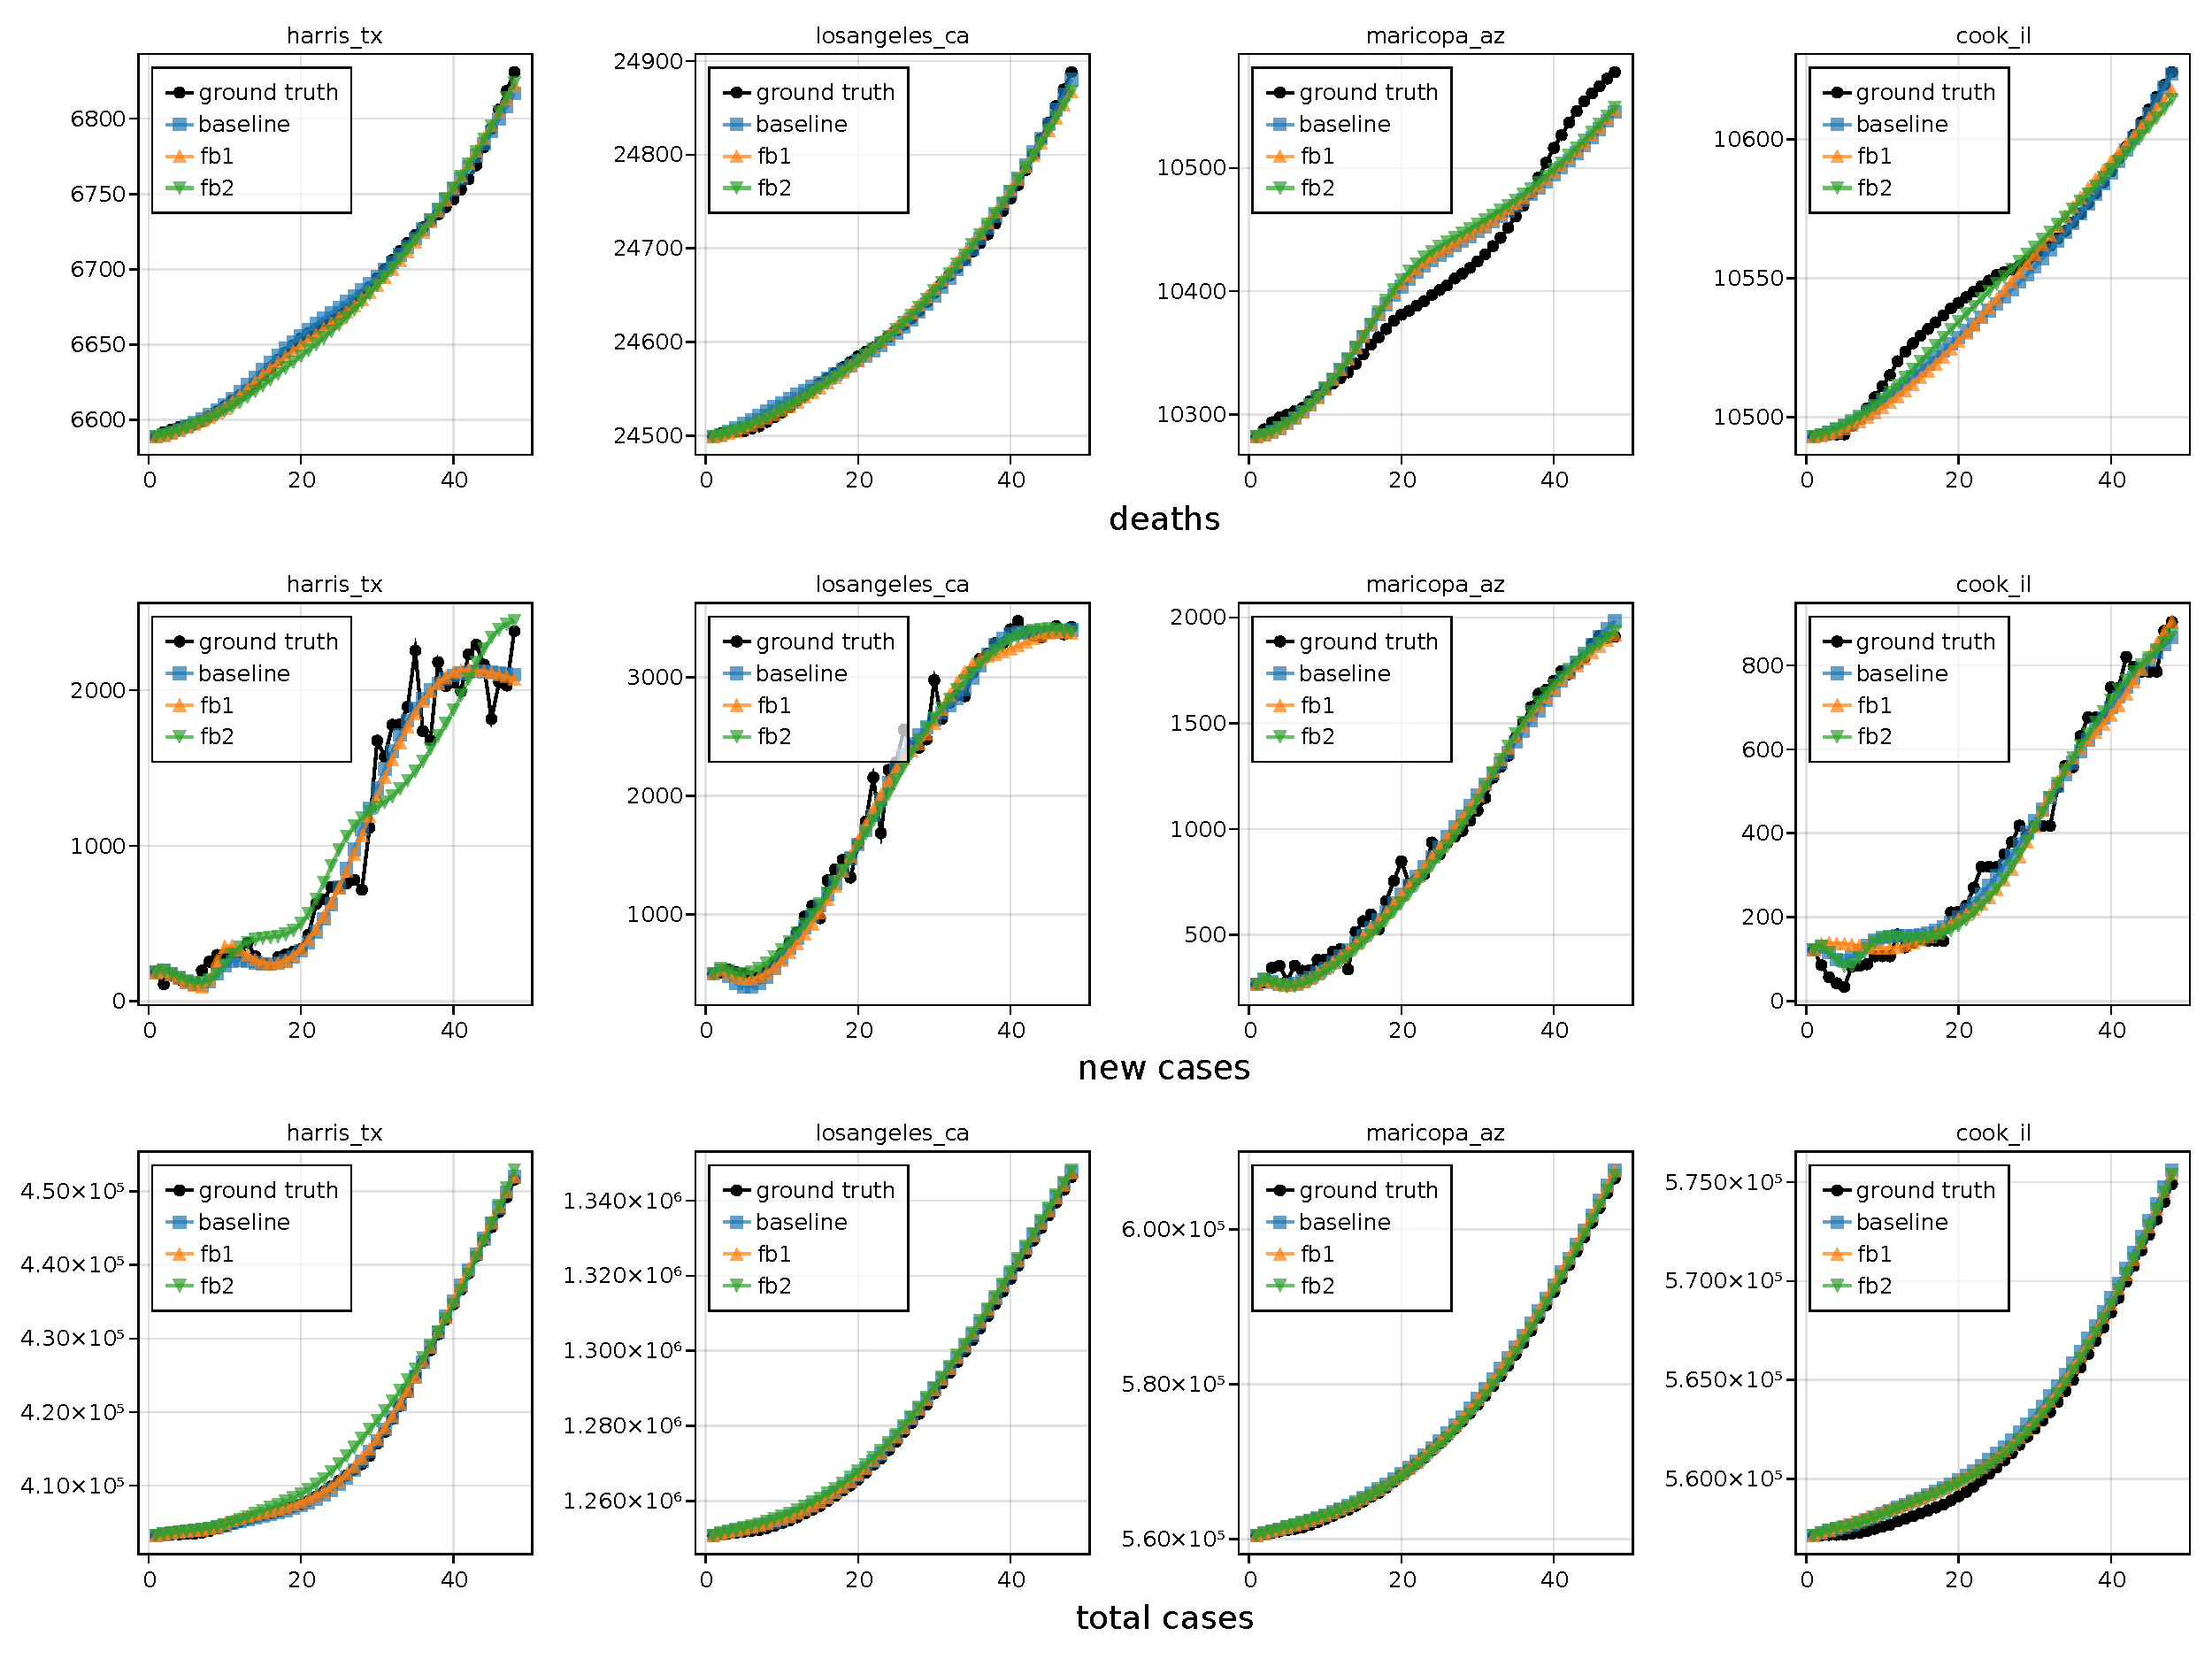
\includegraphics[scale=0.35]{fit_us_counties.pdf}
    \caption{Predictions made by all versions of the model for the training period after having trained with data for \gls{US} counties. Each row contains the predictions for a compartment for each of the considered counties. Here the second version is denoted as \textit{fb1} and the third version is denoted as \textit{fb2}}
    \label{fig:fit-us-counties}
\end{figure}

\begin{figure}[!htb]
    \centering
    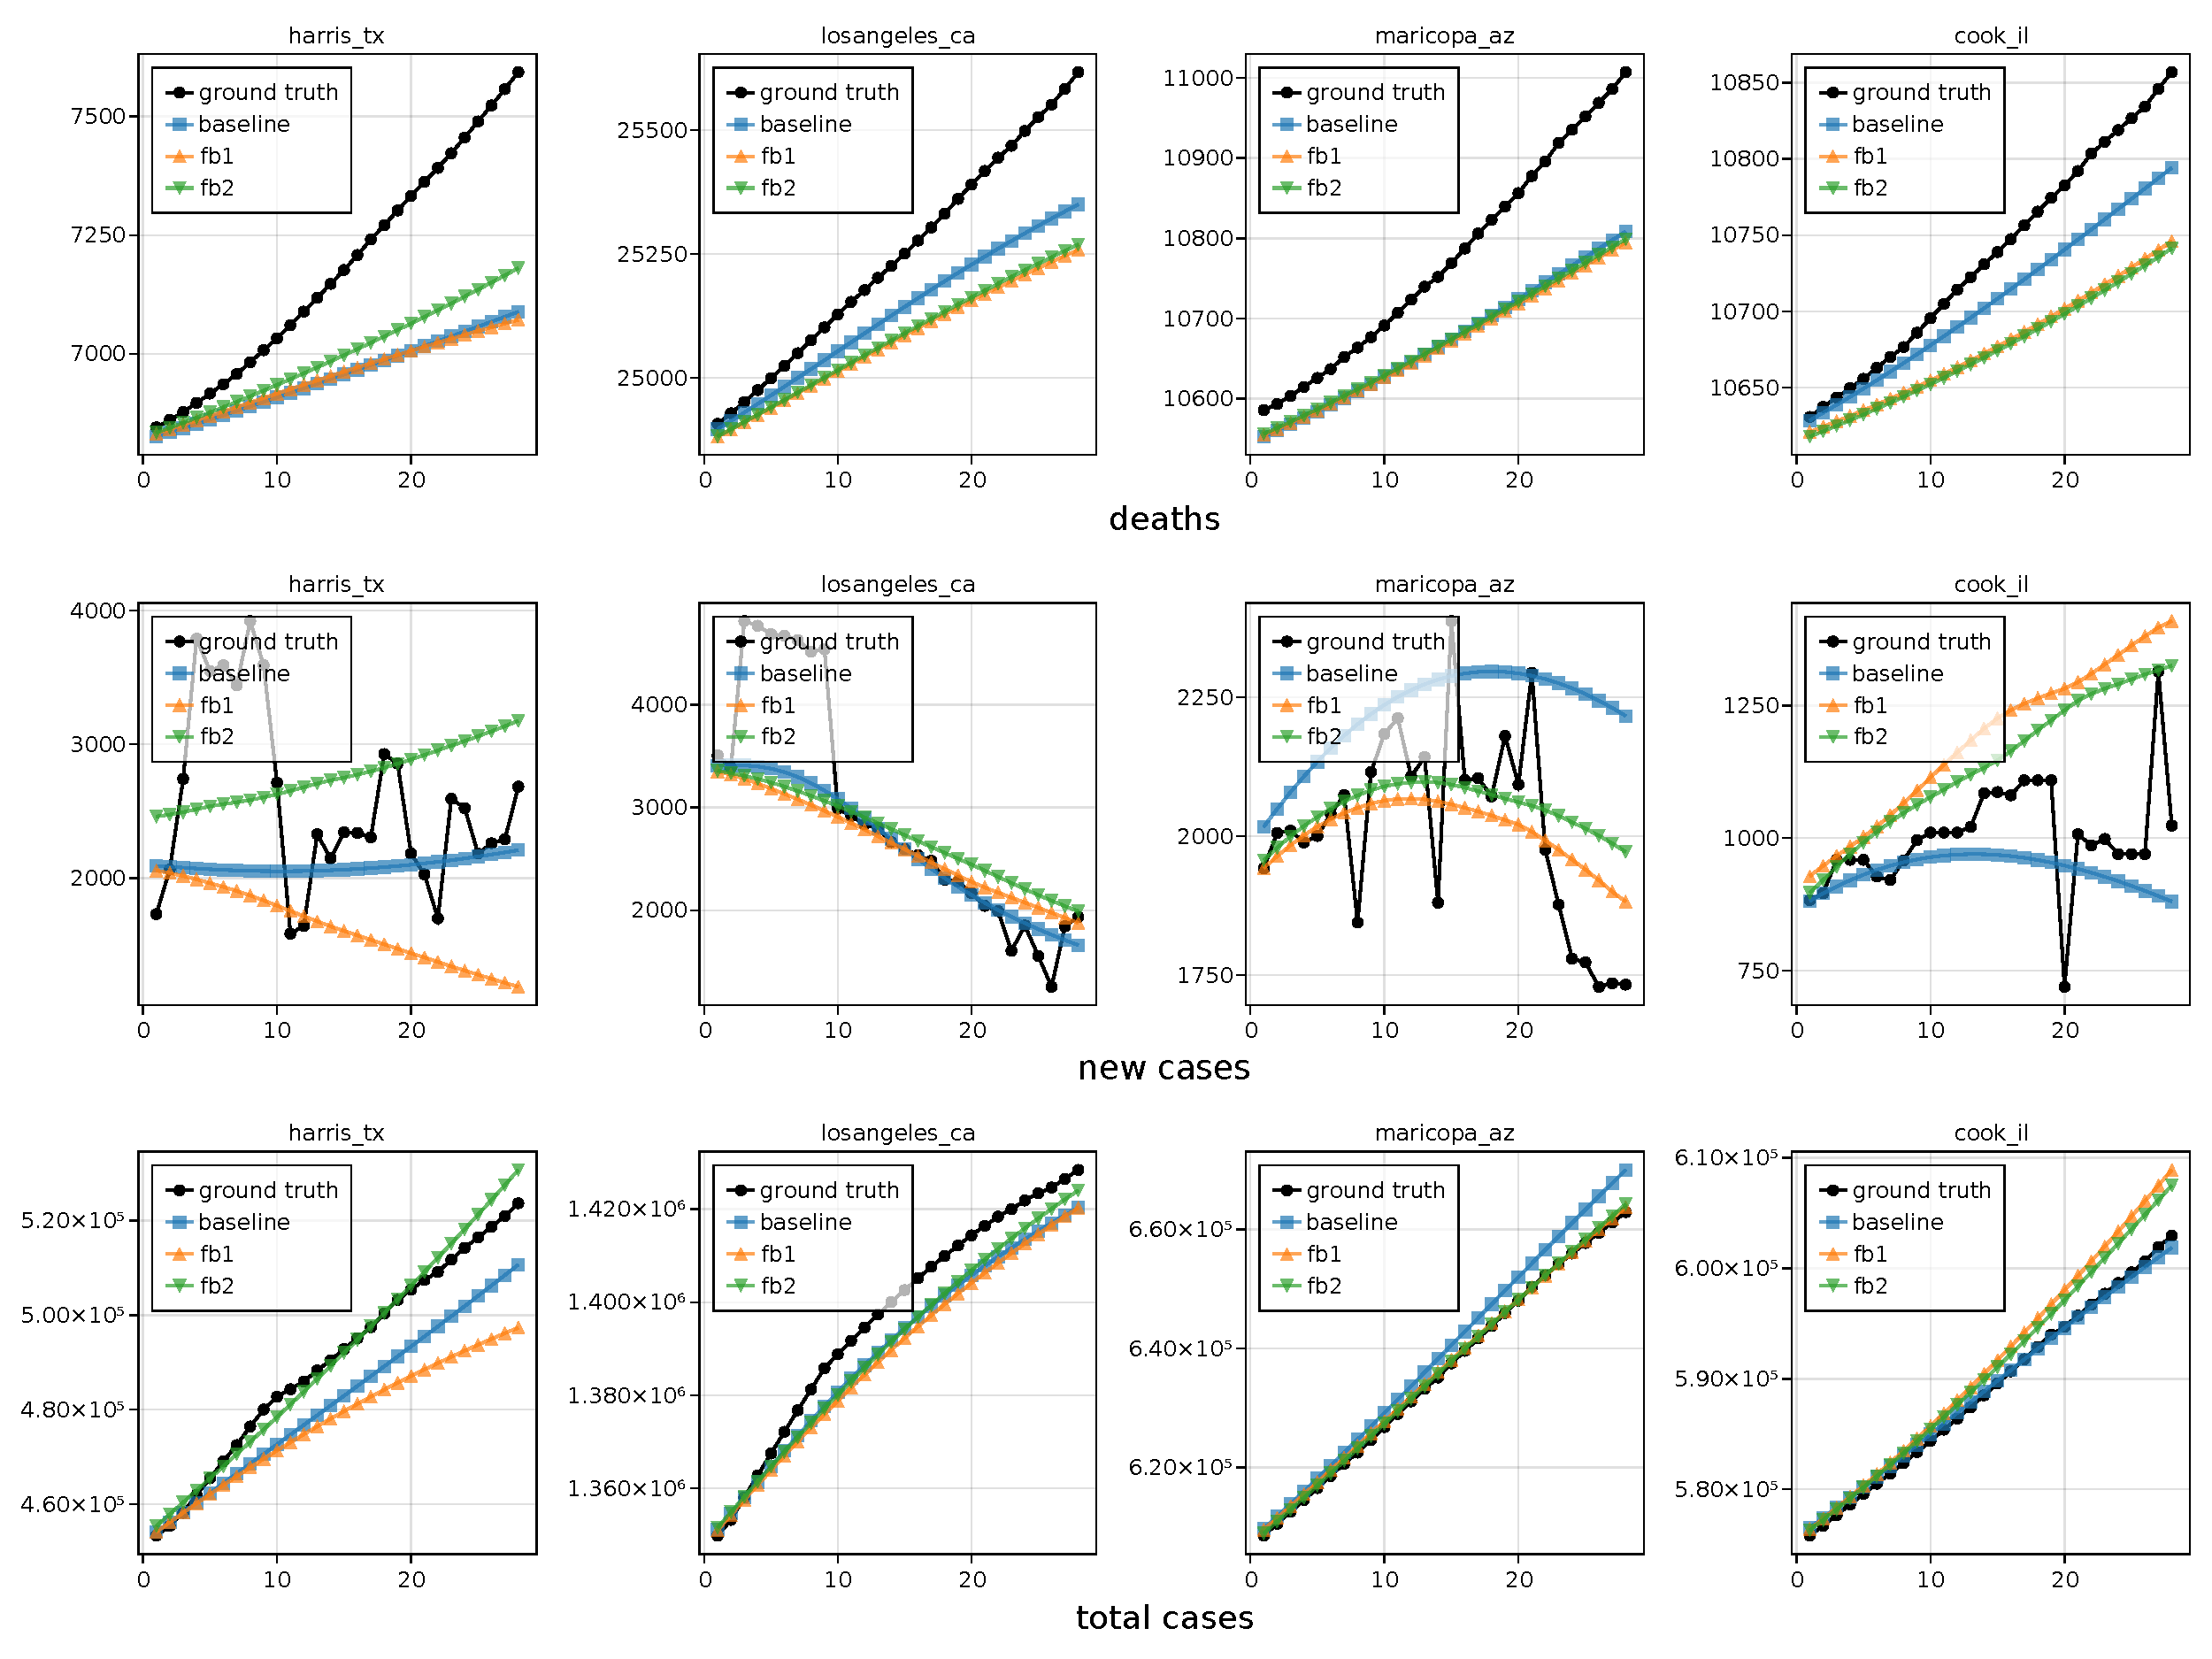
\includegraphics[scale=0.35]{pred_us_counties.pdf}
    \caption{Predictions made by all versions of the model for the testing period after having trained with data for \gls{US} counties. Each row contains the predictions for a compartment for each of the considered counties. Here the second version is denoted as \textit{fb1} and the third version is denoted as \textit{fb2}}
    \label{fig:pred-us-counties}
\end{figure}

\begin{figure}[!htb]
    \centering
    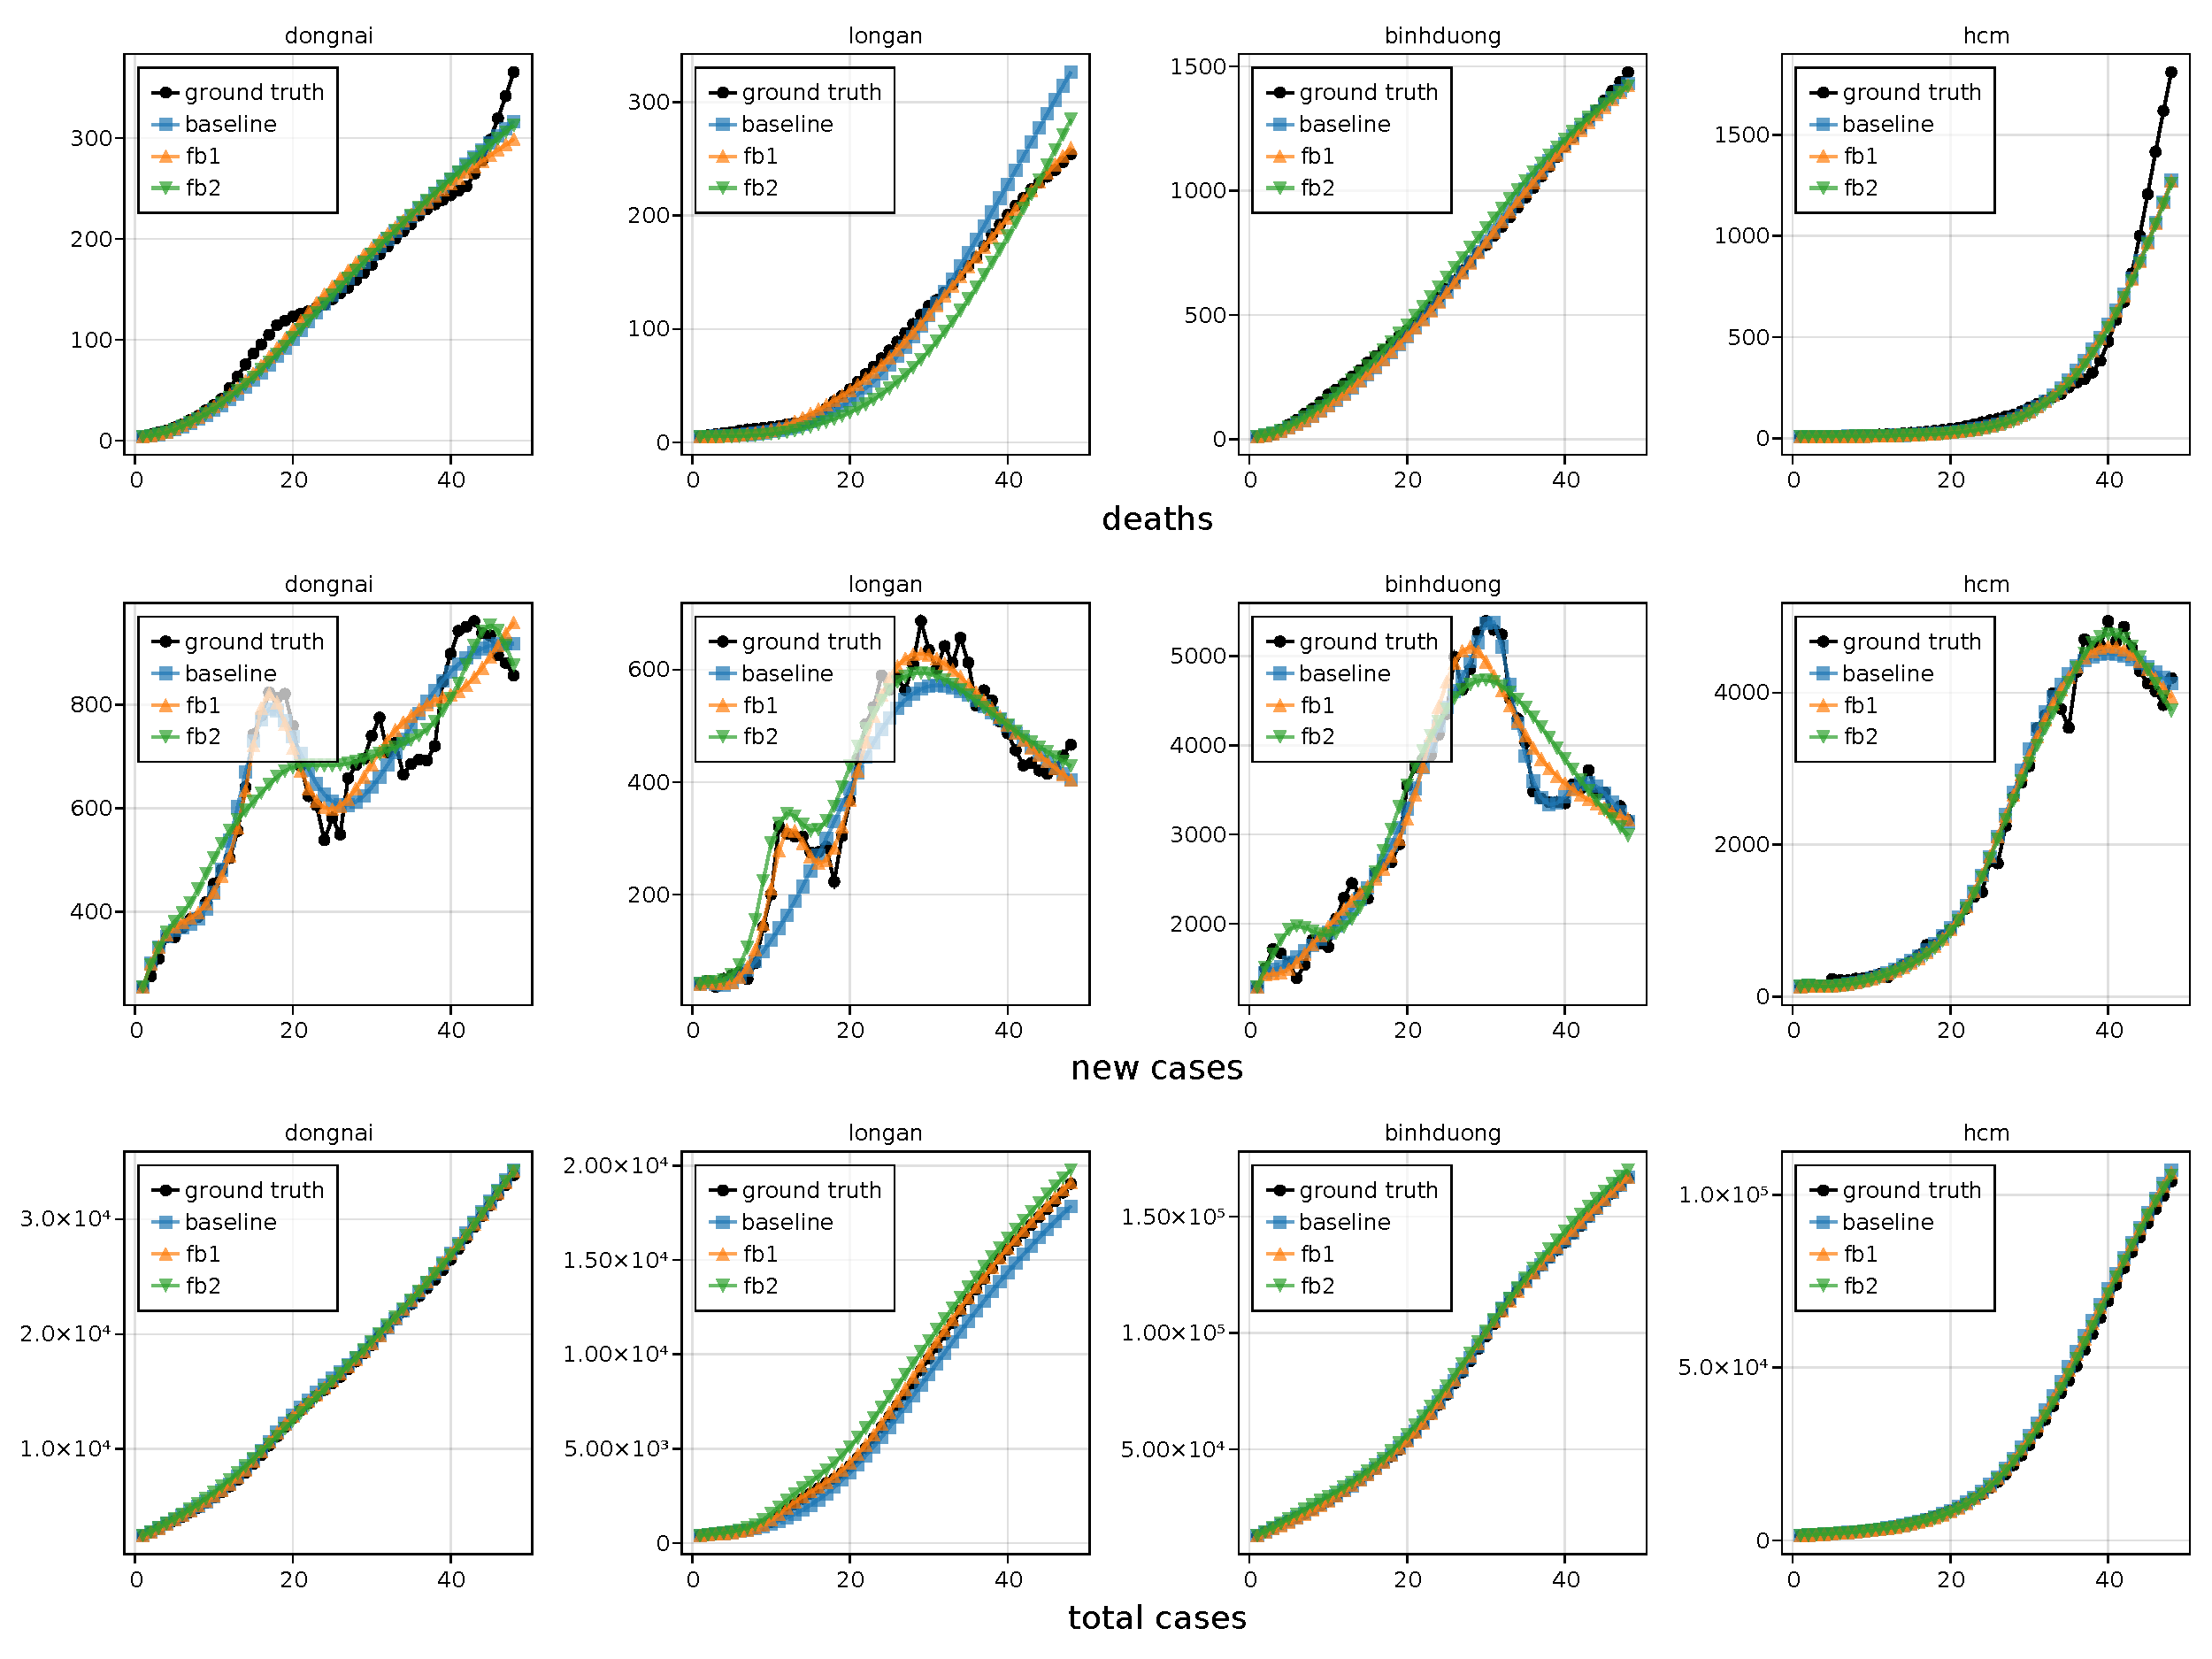
\includegraphics[scale=0.35]{fit_vn_provinces.pdf}
    \caption{Predictions made by all versions of the model for the training period after having trained with data for Vietnam provinces. Each row contains the predictions for a compartment for each of the considered provinces. Here the second version is denoted as \textit{fb1} and the third version is denoted as \textit{fb2}}
    \label{fig:fit-vn-provinces}
\end{figure}

\begin{figure}[!htb]
    \centering
    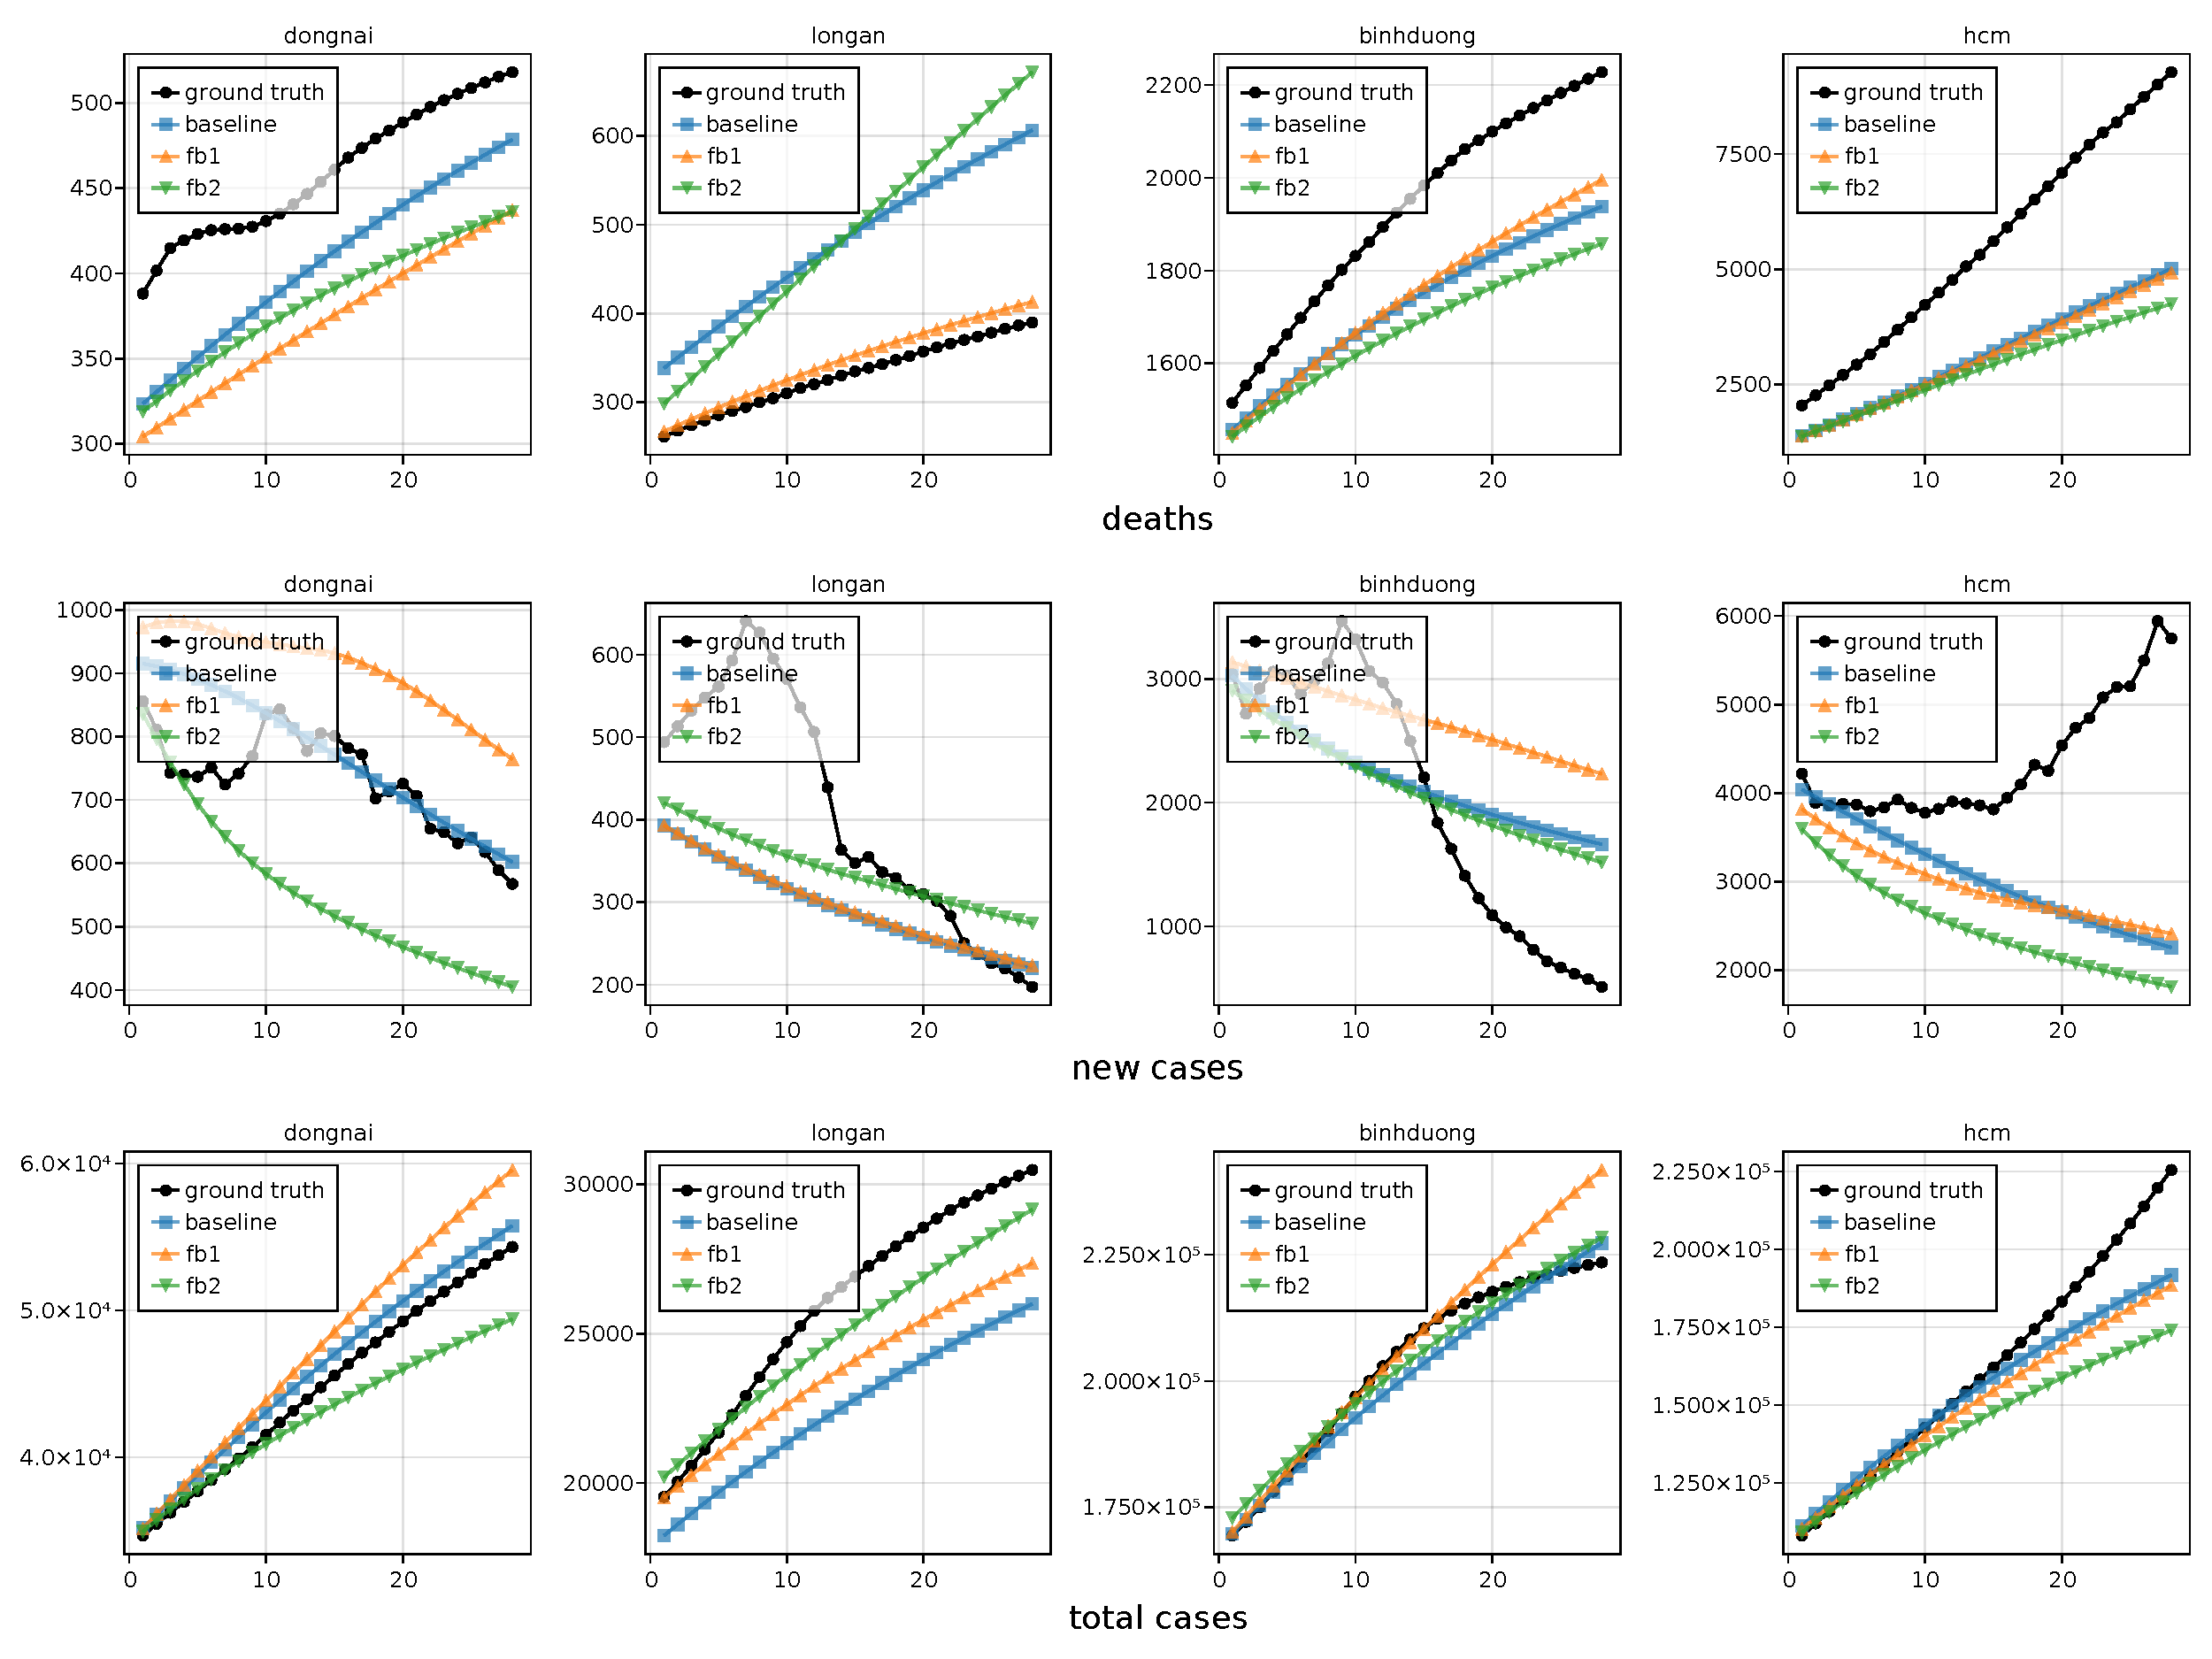
\includegraphics[scale=0.35]{pred_vn_provinces.pdf}
    \caption{Predictions made by all versions of the model for the testing period after having trained with data for Vietnam provinces. Each row contains the predictions for a compartment for each of the considered provinces. Here the second version is denoted as \textit{fb1} and the third version is denoted as \textit{fb2}}
    \label{fig:pred-vn-provinces}
\end{figure}
